\section{Extração de Características}
\label{sec:feature-extraction}

\contentscurrent

\begin{frame}
\frametitle{Características Ideais}
\begin{itemize}
    \item Natural e frequente na fala
    \item Facilmente mensurável
    \item $\uparrow$ variação inter-locutor e $\downarrow$ variação intra-locutor
    \item Constante no tempo e não afetável pela saúde
    \item Robusta a ruído razoável e a transmissão
    \item Difícil de ser produzido artificialmente
    \item Não ser facilmente modificável pelo locutor
\end{itemize}
\end{frame}

\subsection{MFCC}

\begin{frame}
\frametitle{Mel-Frequency Cepstrum Coefficients}
\begin{description}
    \item Simula a função da \textbf{cóclea}
    \item[Escala Mel] Logaritmica
    \begin{itemize}
        \item $f_{mel} = 2595 \log_{10}(1 + \frac{f}{700})$
    \end{itemize}
\end{description}

\begin{figure}[ht]
    \centering
    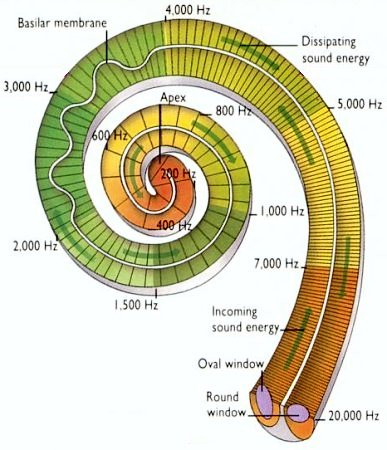
\includegraphics[width=0.35\textwidth]{cochlea}
\end{figure}
\end{frame}

\subsection{MFCC - Extração}

\begin{frame}
\frametitle{MFCC - Extração}
\begin{figure}[ht]
    \centering
    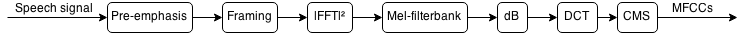
\includegraphics[width=0.75\textwidth]{mfcc-flow}
\end{figure}

\begin{description}
    \item[Pre-emphasis] \textbf{Realça} as frequências altas (opcional)
    \begin{itemize}
        \item $s_{emph}[n] = s[n] - \alpha \cdot s[n - 1]$
        \item $\alpha \in [0.95, 0.98]$, escolhido $\alpha = 0.97$
    \end{itemize}
\end{description}
\begin{figure}[ht]
    \centering
    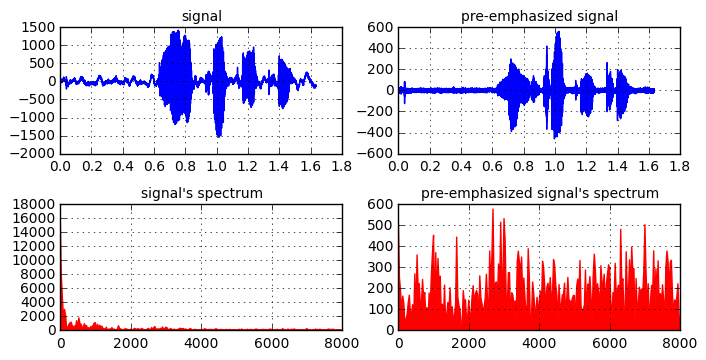
\includegraphics[width=0.75\textwidth]{preemphasis}
\end{figure}
\end{frame}

\subsection{MFCC - Extração}

\begin{frame}
\frametitle{MFCC - Extração}
\begin{figure}[ht]
    \centering
    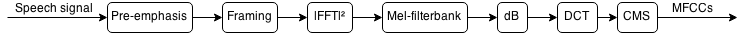
\includegraphics[width=0.75\textwidth]{mfcc-flow}
\end{figure}

\begin{description}
    \item[Framing] Divide o sinal em janelas \textbf{superpostas}
    \begin{itemize}
        \item Janela de Hamming
        \item Largura de 20 milissegundos
        \item Deslocamento de 10 milissegundos
    \end{itemize}
\end{description}
\begin{figure}[ht]
    \centering
    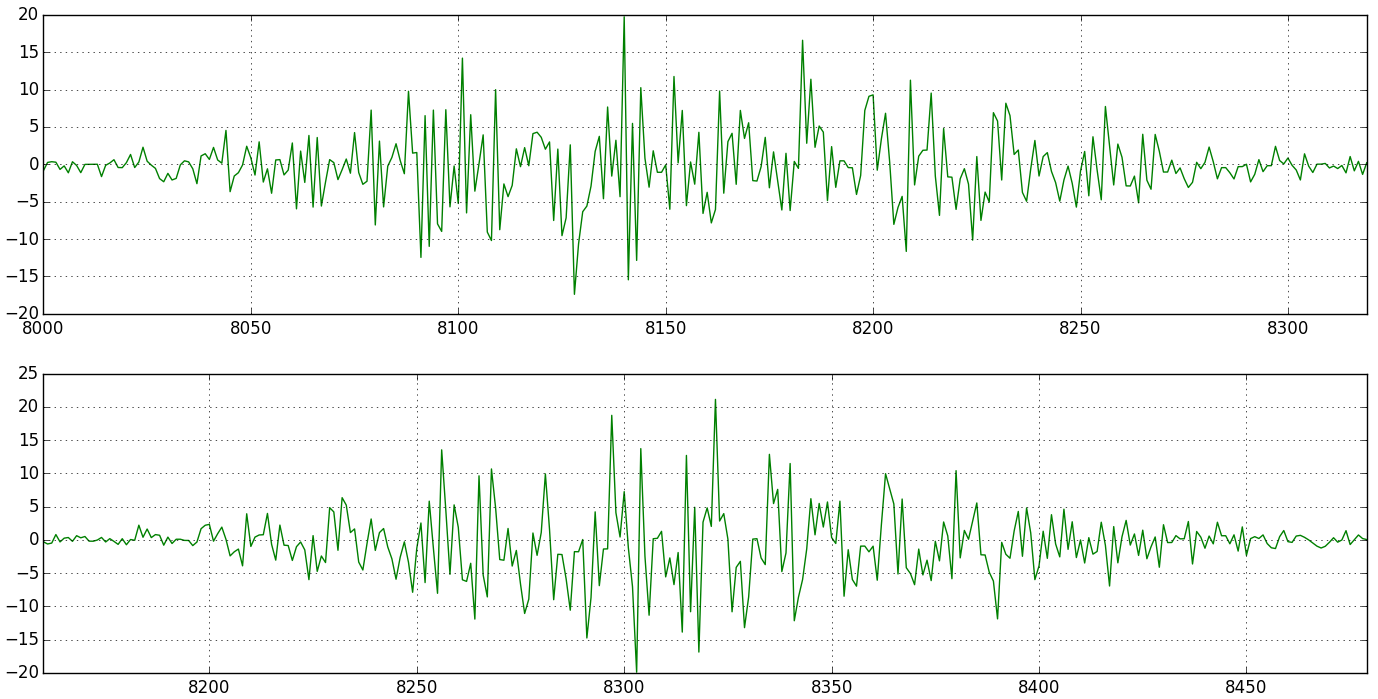
\includegraphics[width=0.75\textwidth]{framing}
\end{figure}
\end{frame}

\subsection{MFCC - Extração}

\begin{frame}
\frametitle{MFCC - Extração}
\begin{figure}[ht]
    \centering
    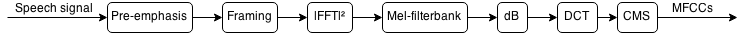
\includegraphics[width=0.75\textwidth]{mfcc-flow}
\end{figure}

\begin{description}
    \item[$|FFT|^2$] Calcula o \textbf{espectro de potência}
\end{description}
\begin{figure}[ht]
    \centering
    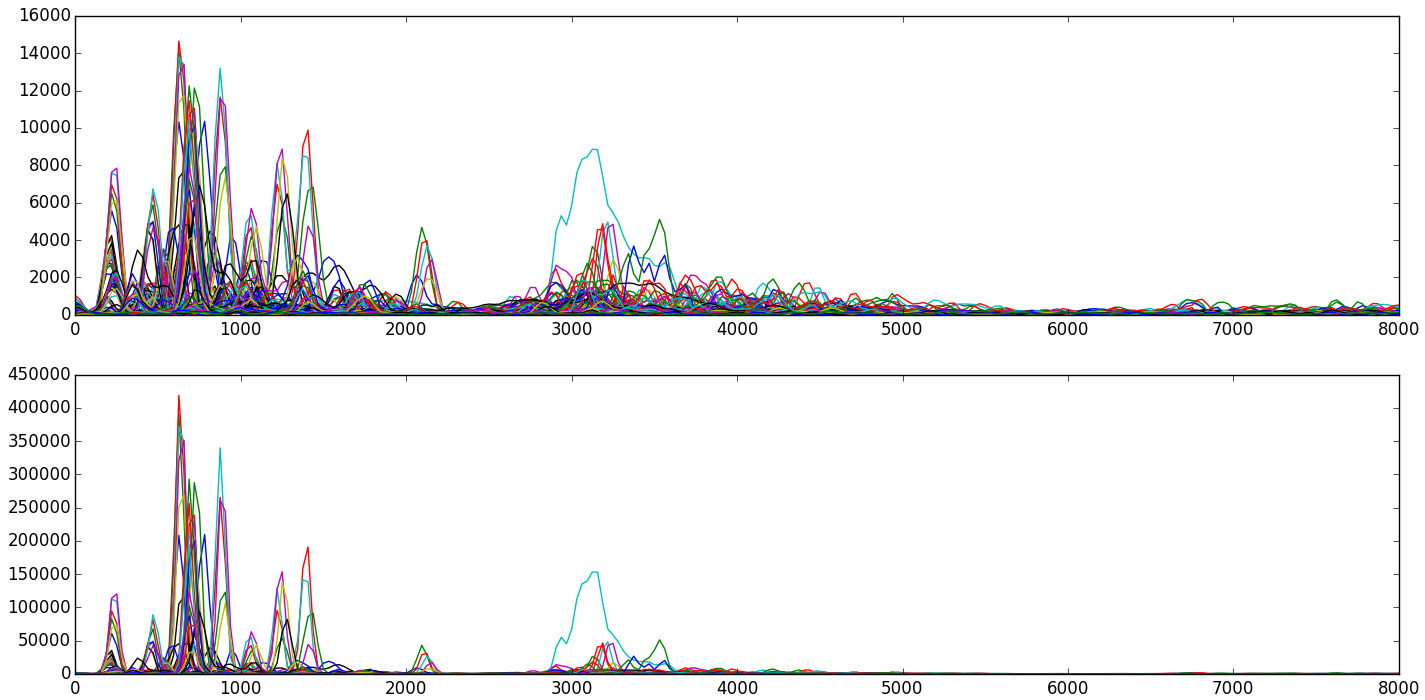
\includegraphics[width=0.6\textwidth]{fft}
\end{figure}
\end{frame}

\subsection{MFCC - Extração}

\begin{frame}
\frametitle{MFCC - Extração}
\begin{figure}[ht]
    \centering
    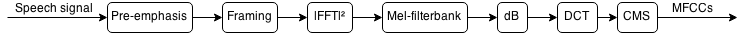
\includegraphics[width=0.75\textwidth]{mfcc-flow}
\end{figure}

\begin{description}
    \item[Mel-filterbank] Espectro em Hz $\implies$ espectro em \textbf{mels}
\end{description}
\begin{figure}[ht]
    \centering
    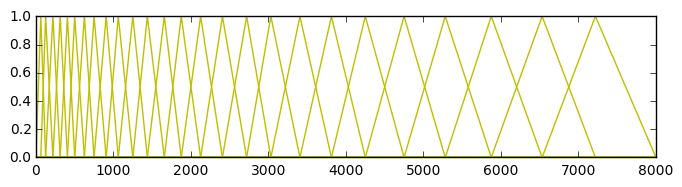
\includegraphics[width=0.75\textwidth]{filterbank}
\end{figure}

\begin{description}
    \item Na escala mel, as larguras são iguais
\end{description}
\end{frame}

\subsection{MFCC - Extração}

\begin{frame}
\frametitle{MFCC - Extração}
\begin{figure}[ht]
    \centering
    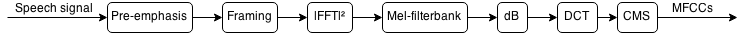
\includegraphics[width=0.75\textwidth]{mfcc-flow}
\end{figure}

\begin{description}
    \item[dB] Calcula a \textbf{sonoridade}
    \begin{itemize}
        \item espectro em mels $\implies$ espectro logarítmico
    \end{itemize}
\end{description}
\begin{figure}[ht]
    \centering
    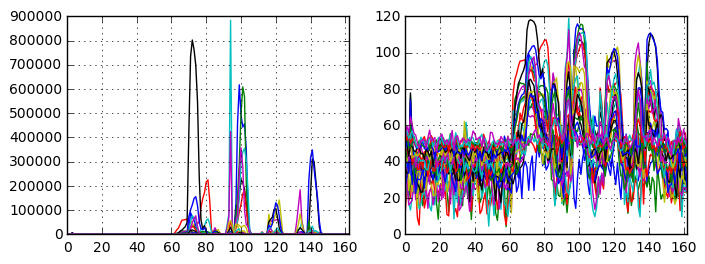
\includegraphics[width=0.75\textwidth]{features_and_featuresdB}
\end{figure}
\end{frame}

\subsection{MFCC - Extração}

\begin{frame}
\frametitle{MFCC - Extração}
\begin{figure}[ht]
    \centering
    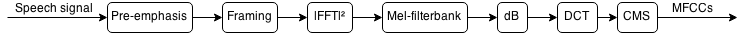
\includegraphics[width=0.75\textwidth]{mfcc-flow}
\end{figure}

\begin{description}
    \item[DCT] Coeficientes espectrais $\implies$ coeficientes \textbf{cepstrais}
    \vskip2pt
    \begin{itemize}
        \item $c_n = \sum_{k=1}^K S_k\cdot\cos\left[n\left(k - \frac{1}{2}\right)\frac{\pi}{K}\right], n = 1, 2, ..., L$
    \end{itemize}
\end{description}
\begin{figure}[ht]
    \centering
    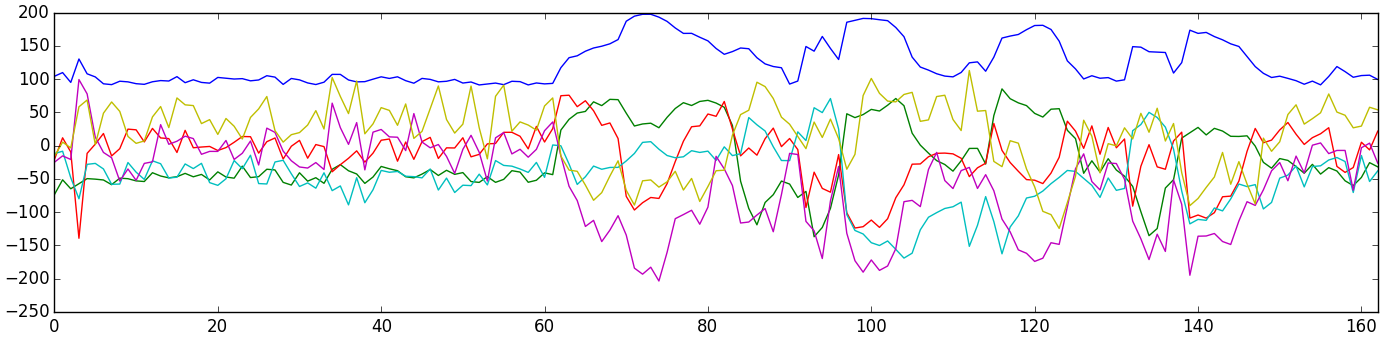
\includegraphics[width=0.7\textwidth]{mfcc}
\end{figure}
\begin{figure}[ht]
    \centering
    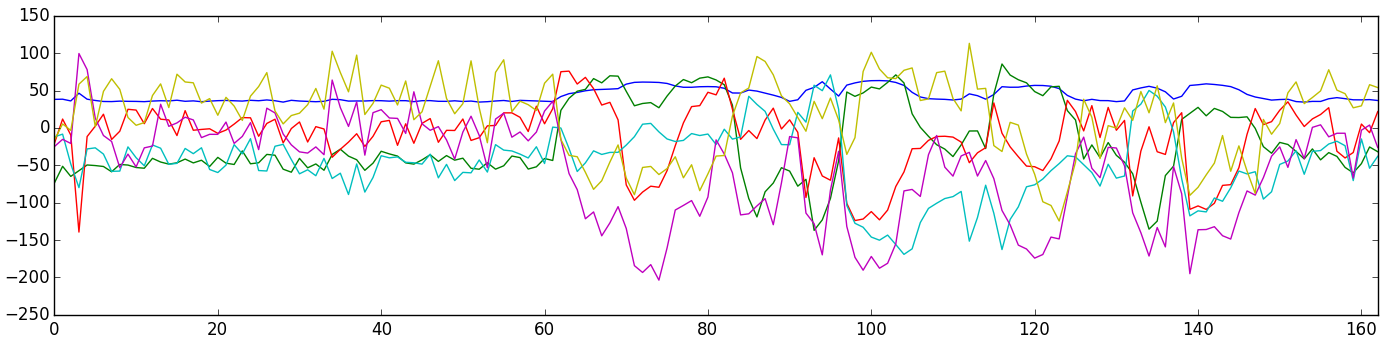
\includegraphics[width=0.7\textwidth]{mfcc_energy_appended}
\end{figure}
\end{frame}

\subsection{MFCC - Extração}

\begin{frame}
\frametitle{MFCC - Extração}
\begin{figure}[ht]
    \centering
    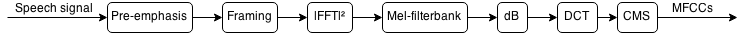
\includegraphics[width=0.75\textwidth]{mfcc-flow}
\end{figure}

\begin{description}
    \item[CMS] \textbf{Normaliza} os MFCCs para reduzir perturbações
    \vskip2pt
    \begin{itemize}
        \item $c_n = c_n - \frac{1}{T} \sum_{t=1}^T c_{n,t}$
    \end{itemize}
\end{description}
\begin{figure}[ht]
    \centering
    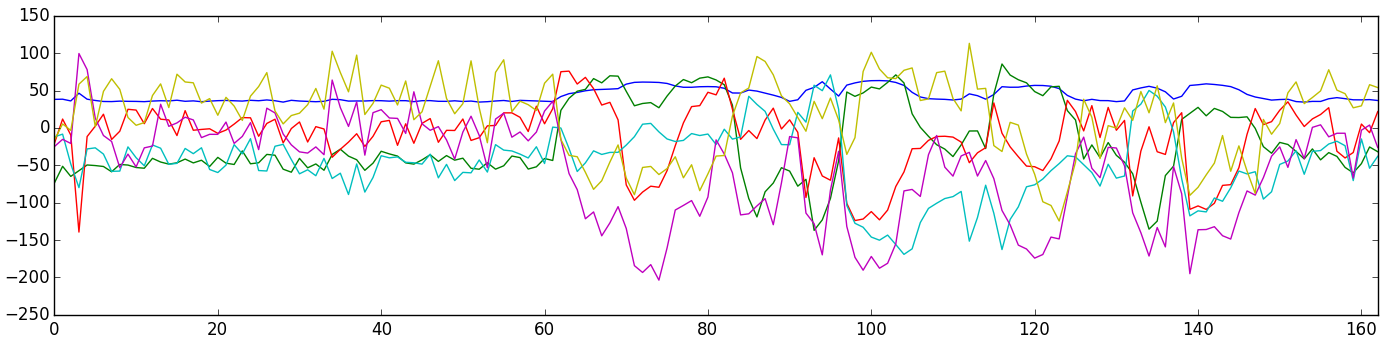
\includegraphics[width=0.7\textwidth]{mfcc_energy_appended}
\end{figure}
\begin{figure}[ht]
    \centering
    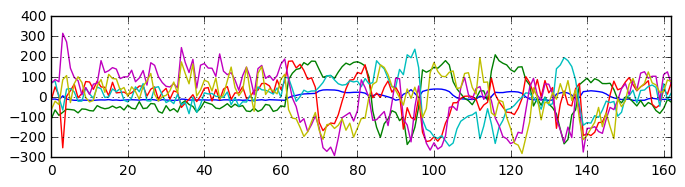
\includegraphics[width=0.7\textwidth]{mfcc_energy_appended_cms}
\end{figure}
\end{frame}

\subsection{MFCC - Extração}

\begin{frame}
\frametitle{MFCC - Extração}
\begin{figure}[ht]
    \centering
    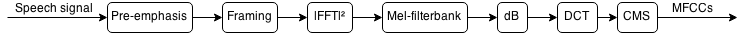
\includegraphics[width=0.75\textwidth]{mfcc-flow}
\end{figure}

\begin{description}
    \item[$\dvec{\Delta}$s] Novos $c_n$ \textbf{derivados} dos antigos $c_n$ (opcional)
    \vskip2pt
    \begin{itemize}
        \item $\Delta_t = \frac{\sum_{n=1}^N n(c_{t+n} - c_{t-n})}{2\sum_{n=1}^N n^2}$
    \end{itemize}
\end{description}
\begin{figure}[ht]
    \centering
    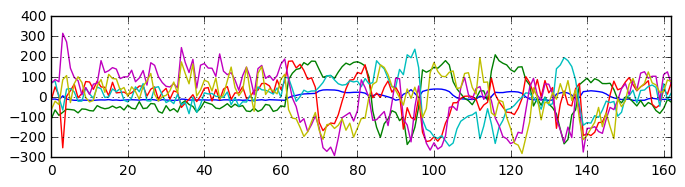
\includegraphics[width=0.7\textwidth]{mfcc_energy_appended_cms}
\end{figure}
\begin{figure}[ht]
    \centering
    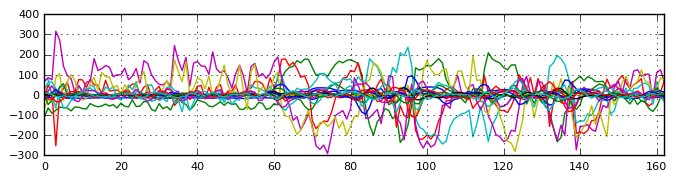
\includegraphics[width=0.7\textwidth]{mfcc_energy_appended_cms_delta_order_2}
\end{figure}
\end{frame}